\newpage
\begin{center}
	\textbf{\large ГЛАВА 6}

	\textbf{\large ВЫЧИСЛИТЕЛЬНЫЕ ЭКСПЕРИМЕНТЫ}
\end{center}
\refstepcounter{chapter}
\addcontentsline{toc}{chapter}{6. ВЫЧИСЛИТЕЛЬНЫЕ ЭКСПЕРИМЕНТЫ}

\section{Синтетические задачи}

В начале исследования, для проверки применимости и практической полезности описанных в \textit{Главе 1} релятивистских матриц косинусов (прежде всего \ref{C_rel_definition_practical}), были предложены несколько экспериментов, с использованием данных матриц. Все они предполагали генерацию случайной двумерной или трёхмерной цепи, а после рассчёт некоторой заданной функции (скалярной, векторной) в точках вокруг этой цепи. Потом обучалась полносвёрточная нейронная сеть для аппроксимации заданной функции, -- нейронную сеть учили по матрице \ref{C_rel_definition_practical} предсказывать некоторое, тоже матричное, представление значения функции.

Эти эксперименты показали, что новые предложенные матрицы косинусов фундаментально подходят для представления некоторой ломаной и точки в пространстве, и такое представление может использоваться как входные данные для нейронных сетей.

\subsection{Задача №1}
В первой задачу функция задавалась следующим образом. Пусть $a_i$, $i=\overline{1,n}$ -- координаты точек случайной цепи, и $c$ -- некоторый малый параметр, тогда:
\begin{equation}
	f(x) = \sum_{i=1}^n\frac{1}{||x - a_i||\mathbb{I}[||x - a_i|| < c] + c\mathbb{I}[||x - a_i|| \ge c]}.
	\label{synt1_f}
\end{equation}
Для обучения нейронной сети использовались случайные точки из многомерного нормального распределения. При суммировании квадрат отклонения предсказания от истинной $f(x)$ делился на плотность распределения и усреднялся (см. \ref{monte-carlo2}). Значение функции - скаляр, поэтому он кодировался как в \ref{scalar_F}.

\subsection{Задача №2}
Во второй задаче целью было извлечение из релятивистской матрицы косинусов координат закодированной точки. Нейронная сеть предсказывала обычную матрицу косинусов вида \ref{C_nu_definition}, которая кодировала вектор из центра цепи к извлекаемой точке.
\begin{figure}[H]
	\centering
	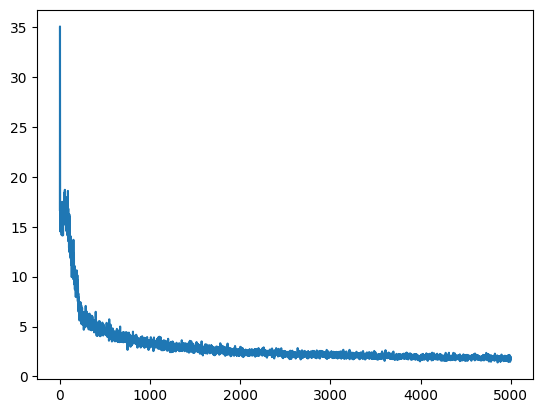
\includegraphics[scale=0.5]{rel2train.png}
	\caption{График функции потерь при решении задачи №2.}
	\label{fig_synt2_train}
\end{figure}
\begin{figure}[H]
	\centering
	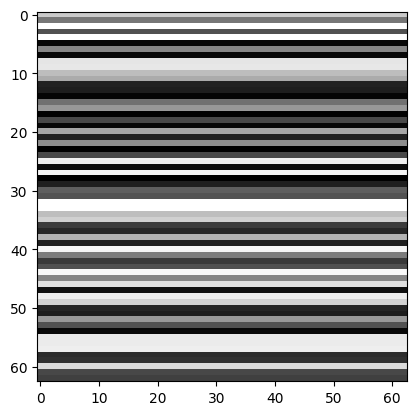
\includegraphics[scale=0.5]{rel21.png}
	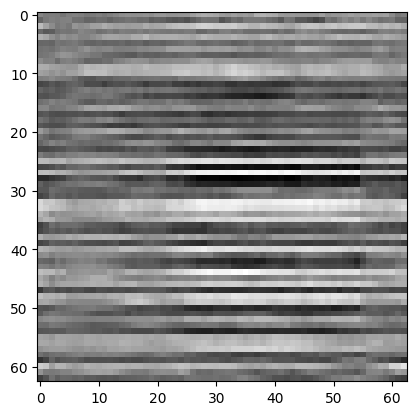
\includegraphics[scale=0.5]{rel22.png}
	\caption{Истинная и предсказанная $C_{\nu}$.}
	\label{fig_synt2_1}
\end{figure}
\begin{figure}[H]
	\centering
	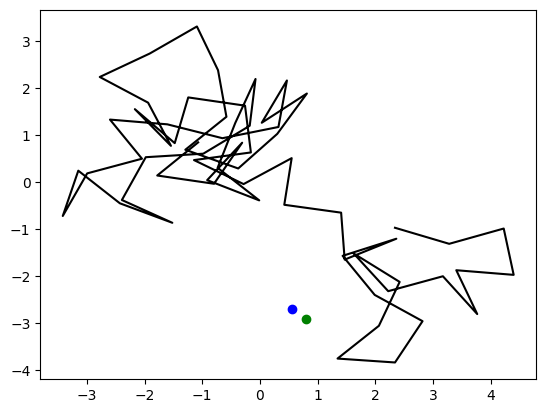
\includegraphics[scale=0.5]{rel23.png}
	\caption{Настоящая (зелёная) и предсказанная (синяя) позиция точки.}
	\label{fig_synt2_2}
\end{figure}

\subsection{Задача №3}
Эта задача является векторной модификацией \textit{Задачи №1}, то есть вместо суммы скалярных значений, складывались векторы.
\begin{figure}[H]
	\centering
	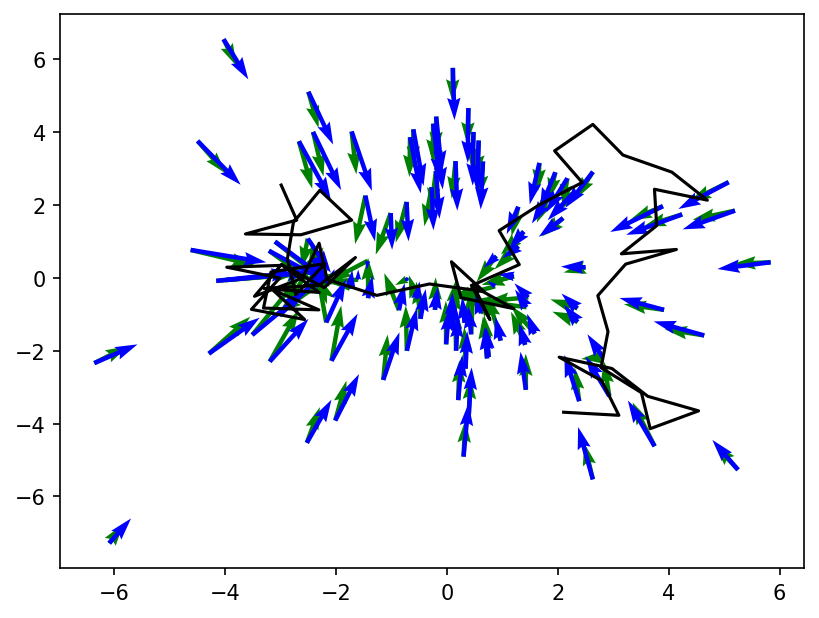
\includegraphics[scale=0.75]{rel31.png}
	\caption{Настоящие (зелёные) и предсказанные (синие) векторы.}
	\label{fig_synt3}
\end{figure}

\subsection{Задача №4}
Эта задача также является модификацией \textit{Задачи №1}. В ней значения \ref{synt1_f} большие некоторой заданной константы заменяются 1, а меньшие -- 0. Такая функция позволяет создать некоторую оболочку вокруг ломаной $a_i$. Такие оболочки крайне нужны, так как процедура обучения нейронных сетей, описанная в предыдущей главе, не учит нейронные сети занулять поле в удалённых от молекулы участках. При свободном моделировании с использованием методик из \textit{Главы 4}, иметь такую функцию оболочку крайне необходимо. Впрочем, использования для этой цели целой нейросети представляет, разве что, теоретический интерес.
\begin{figure}[H]
	\centering
	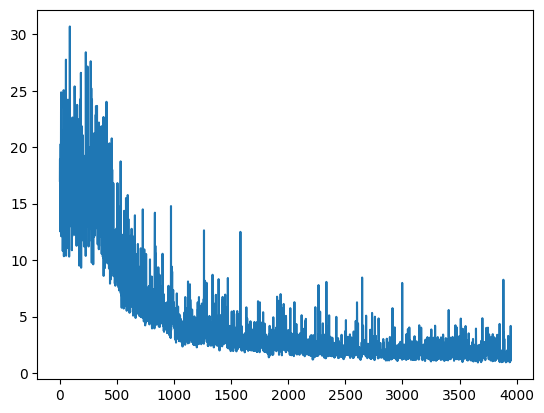
\includegraphics[scale=0.5]{rel4train.png}
	\caption{График функции потерь при решении задачи №4.}
	\label{fig_synt3_train}
\end{figure}
\begin{figure}[H]
	\centering
	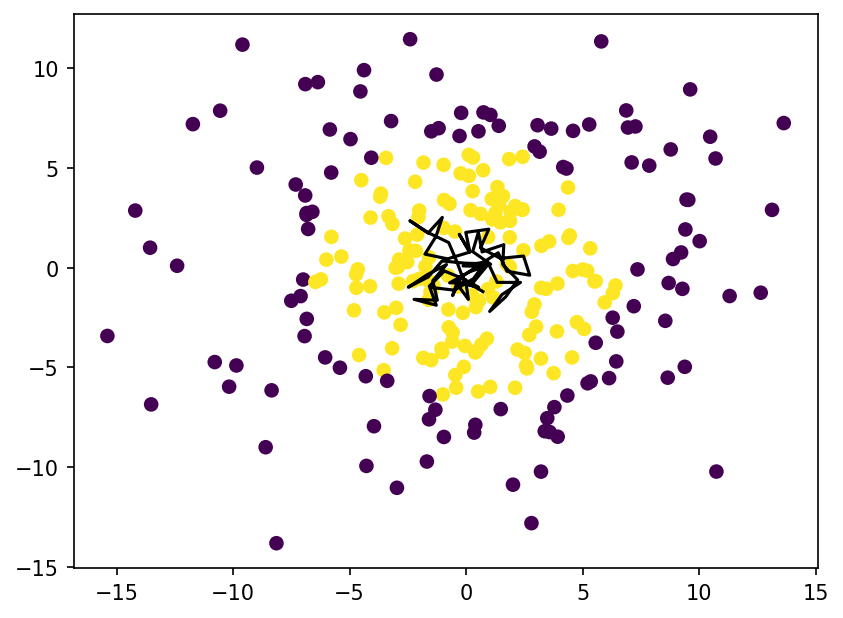
\includegraphics[scale=0.5]{rel42.png}
	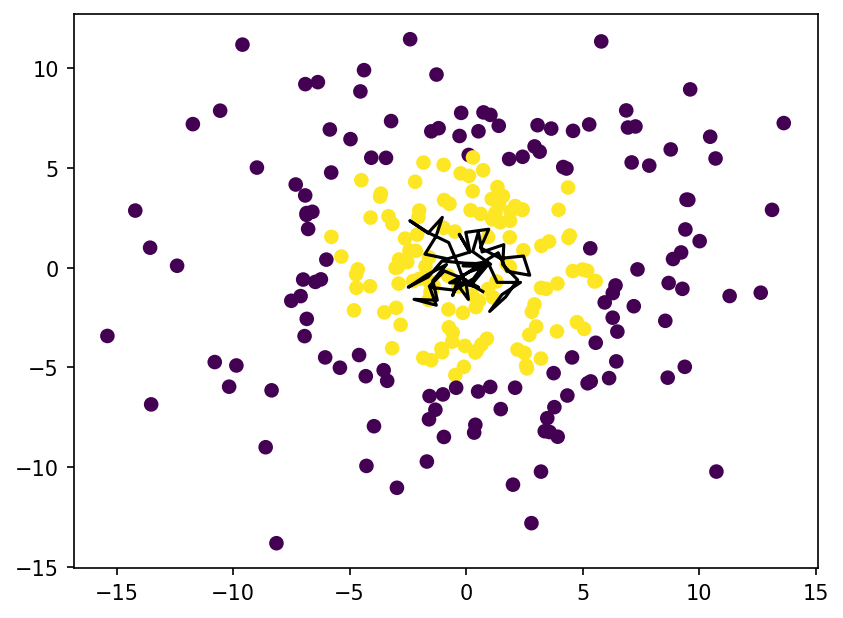
\includegraphics[scale=0.5]{rel43.png}
	\caption{Истинная и предсказанная оболочки.}
	\label{fig_synt4}
\end{figure}

\section{Моделирование полей для задачи взаимодействия белков}

Для получения поля, моделирующего белок-белковое взаимодействие, были использованы архитектура и протокол обучения из \textit{Главы 5}. Были опробованы скалярные \ref{L_multiscalar}, векторные \ref{L_scalar_vec} и матричные \ref{mtrx_lagr} формы функции Лагранжа.
\begin{figure}[H]
	\centering
	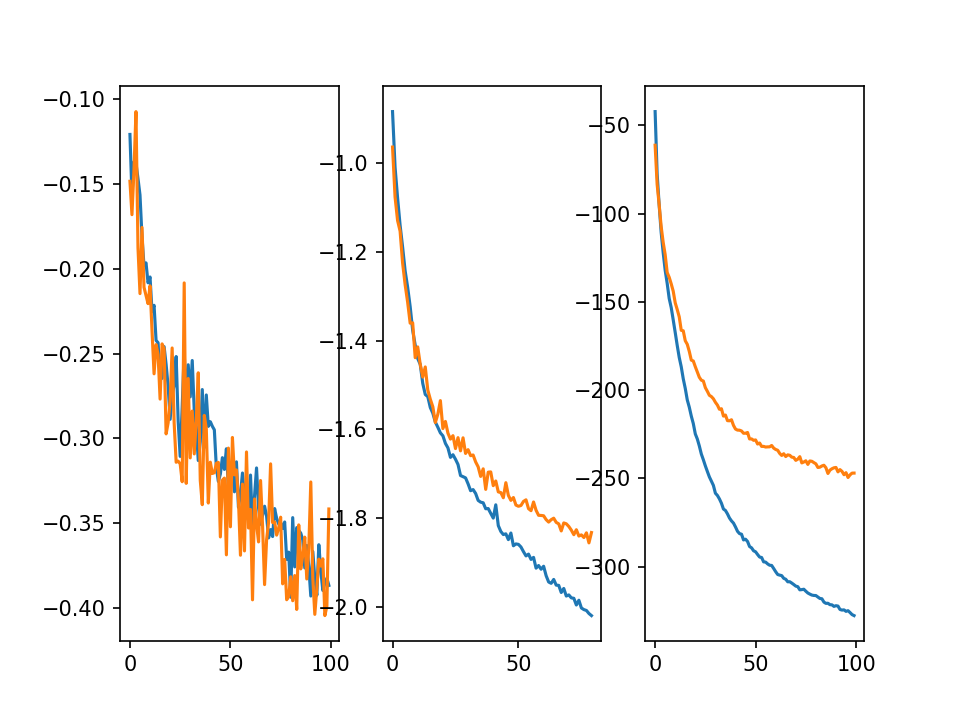
\includegraphics[scale=0.8]{train_plots.png}
	\caption{Графики функции потерь для (слева-направо) мультискалярного, мультивекторного и мультиматричного лагранжиана. Синий -- обучающая выборка, красный -- тестовая.}
	\label{fig_train_plots}
\end{figure}
Наибольший успех был достигнут при исследовании матричных и мультиматричных лагранжианов, однако при нем заметно наличие некоторого переобучения. Наиболее просто обучать мультискалярные функции Лагранжа, однако, как можно видеть по рисунку \ref{fig_train_plots}, их обучение крайне нестабильно, а дальнейший анализ показал их совсем невысокую практичность. В то же время, для них практически не видно какого-либо переобучения. 

\subsection{Анализ лучшей модели}
Наилучшей моделью оказалась мультискалярная модель, являвшаяся суммой 8 полей (1 поле было нулевым и использовалось для нормализации значения других полей). Использовалась нейронная сеть FCN5 с сокращённым числом каналов. Интегрирование по пространству с использованием \ref{logit_fourier} оказалось здесь неэффективным, из-за большого разброса значений частичного лагранжиана в разных точках пространства (приближение оказалось слишком гладким).

Интегрированание по интерфейсу выглядит адекватно, причём для истинных моделей практически всегда имеем довольно низкие значения частичного лагранжиана, и с крайне высокой вероятностью ниже, чем для случайной ложной модели. Однако тут и возникает основная проблема: было замечено, что фактически для любой пары молекул, находилась ложная модель, имевшая более низкое значение частичного лагранжиана. Поэтому был проведён статистический анализ, в котором для каждой пары молекул строилось выборочное распределение лагранжиана, и замерялся квантиль истинного значения:
\begin{figure}[H]
	\centering
	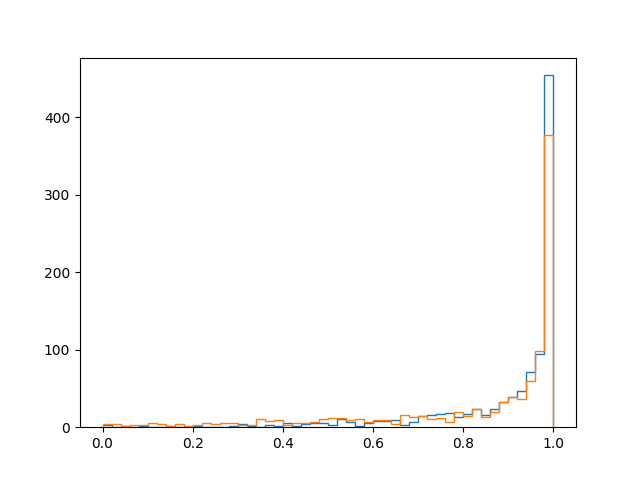
\includegraphics[scale=0.7]{perc.png}
	\caption{Квантиль истинного значения лагранжиана для обучающей (синий) и тестовой (красный) выборок. Значение в 1 означает, что истинное значение также и минимальное.}
	\label{fig_perc}
\end{figure}
Кроме того, эти ложные модели в подавляющем большинстве случаев совершенно непохожи на истинные:
\begin{figure}[H]
	\centering
	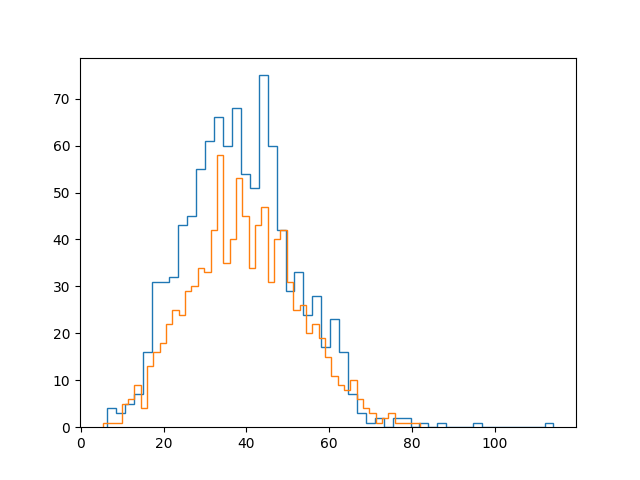
\includegraphics[scale=0.7]{rmsd.png}
	\caption{RMSD между истинной и лучшей моделями взаимодействия для обучающей (синий) и тестовой (красный) выборок.}
	\label{fig_rmsd}
\end{figure}
Несмотря на это, истинные значения частичного лагранжиана практически всегда отрицательны, и довольно низки, в то же время как соответствующие случайные распределения довольно симметричны относительно 0:
\begin{figure}[H]
	\centering
	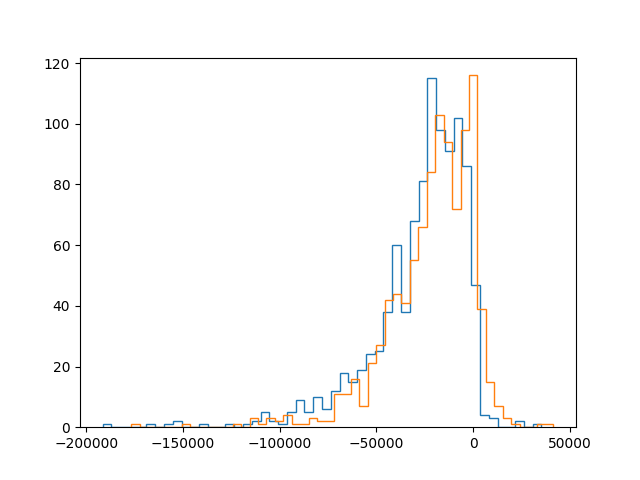
\includegraphics[scale=0.7]{trueval.png}
	\caption{Истинные значения частичного лагранжиана для обучающей (синий) и тестовой (красный) выборок.}
	\label{fig_trueval}
\end{figure}

Основной вывод который можно отсюда сделать заключается в том, что в целом, предложенный подход имеет право на существование, так как нейронная сеть всё же справляется с тем, чтобы получить некоторые представления о белок-белковых взаимодействиях. Слабым местом, по всей видимости, является процедура обучения -- она не гарантирует глобальной минимальности для истинных моделей комплексов. Кроме того, можно попробовать соединить данную модель с некоторой иной моделью машинного обучения через веса в \ref{interface_integral_weight}.